\chapter{Pro and Con}

At the period when these events took place, I had just returned
from a scientific research in the disagreeable territory
of Nebraska, in the United States.  In virtue of my office
as Assistant Professor in the Museum of Natural History in Paris,
the French Government had attached me to that expedition.
After six months in Nebraska, I arrived in New York towards
the end of March, laden with a precious collection.
My departure for France was fixed for the first days in May.
Meanwhile I was occupying myself in classifying my mineralogical,
botanical, and zoological riches, when the accident happened
to the Scotia.

I was perfectly up in the subject which was the question of the day.
How could I be otherwise?  I had read and reread all the American
and European papers without being any nearer a conclusion.
This mystery puzzled me.  Under the impossibility of forming
an opinion, I jumped from one extreme to the other.
That there really was something could not be doubted,
and the incredulous were invited to put their finger on the wound
of the Scotia.\cite{incollection-full}

\section{An added section}

On my arrival at New York the question was at its height.
The theory of the floating island, and the unapproachable sandbank,
supported by minds little competent to form a judgment, was abandoned.
And, indeed, unless this shoal had a machine in its stomach,
how could it change its position with such astonishing rapidity?

From the same cause, the idea of a floating hull of an enormous
wreck was given up.

\vskip 0.25in
\begin{table}%
 \caption[Add a table]{Add an extra table here. Chinese Menu.}
 \begin{center}
  \begin{tabular}{lp{4.4cm}p{4.4cm}}
                & \textbf{column A} & \textbf{column B} \\
  \textbf{hot}  & Kung Pao Chicken  & General Tso's Chicken \\
  \textbf{mild} & Moo Goo Gai Pan   & Sweet and Sour Pork
  \end{tabular}
  \label{tab:test1}
 \end{center}
\end{table}

There remained, then, only two possible solutions of the question,
which created two distinct parties:  on one side, those who were
for a monster of colossal strength; on the other, those who were
for a submarine vessel of enormous motive power.

\subsection{A subsection}

But this last theory, plausible as it was, could not stand against
inquiries made in both worlds.  That a private gentleman should have
such a machine at his command was not likely.  Where, when, and how
was it built? and how could its construction have been kept secret?
Certainly a Government might possess such a destructive machine.
And in these disastrous times, when the ingenuity of man has
multiplied the power of weapons of war, it was possible that,
without the knowledge of others, a State might try to work such
a formidable engine.

But the idea of a war machine fell before the declaration of Governments.
As public interest was in question, and transatlantic communications
suffered, their veracity could not be doubted.  But how admit that
the construction of this submarine boat had escaped the public eye?
For a private gentleman to keep the secret under such circumstances would
be very difficult, and for a State whose every act is persistently watched
by powerful rivals, certainly impossible.

\begin{figure}%
  \centering%
    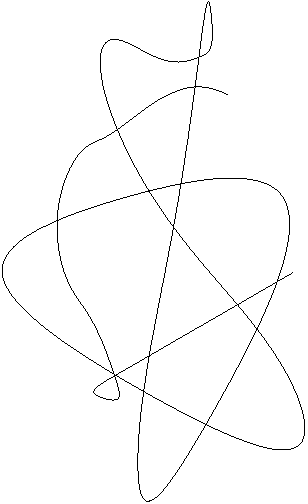
\includegraphics[width=100bp]{jules-verne-test}%
  \caption[Another test figure]%
  {This is another test figure inserted into this text
\protect\cite{misc-full}}%
  \label{fig:test2}%
\end{figure}

Upon my arrival in New York several persons did me
the honour of consulting me on the phenomenon in question.
I had published in France a work in quarto, in two volumes,
entitled Mysteries of the Great Submarine Grounds.  This book,
highly approved of in the learned world, gained for me a special
reputation in this rather obscure branch of Natural History.
My advice was asked.  As long as I could deny the reality
of the fact, I confined myself to a decided negative.
But soon, finding myself driven into a corner, I was
obliged to explain myself point by point.  I discussed
the question in all its forms, politically and scientifically;
and I give here an extract from a carefully-studied article
which I published in the number of the 30th of April.
It ran as follows:

\section{Another added section}

``After examining one by one the different theories, rejecting all
other suggestions, it becomes necessary to admit the existence
of a marine animal of enormous power.

\begin{equation}
E=mc^2
\end{equation}

``The great depths of the ocean are entirely unknown to us.
Soundings cannot reach them.  What passes in those remote depths---what 
beings live, or can live, twelve or fifteen miles beneath
the surface of the waters---what is the organisation of these animals,
we can scarcely conjecture.  However, the solution of the problem
submitted to me may modify the form of the dilemma.  Either we do know
all the varieties of beings which people our planet, or we do not.
If we do NOT know them all---if Nature has still secrets in the deeps
for us, nothing is more conformable to reason than to admit the existence
of fishes, or cetaceans of other kinds, or even of new species,
of an organisation formed to inhabit the strata inaccessible to soundings,
and which an accident of some sort has brought at long intervals
to the upper level of the ocean.

``If, on the contrary, we DO know all living kinds, we must
necessarily seek for the animal in question amongst those marine
beings already classed; and, in that case, I should be disposed
to admit the existence of a gigantic narwhal.

``The common narwhal, or unicorn of the sea, often attains
a length of sixty feet.  Increase its size fivefold or tenfold,
give it strength proportionate to its size, lengthen its
destructive weapons, and you obtain the animal required.
It will have the proportions determined by the officers
of the Shannon, the instrument required by the perforation
of the Scotia, and the power necessary to pierce the hull
of the steamer.\cite{inproceedings-full}

``Indeed, the narwhal is armed with a sort of ivory sword,
a halberd, according to the expression of certain naturalists.
The principal tusk has the hardness of steel.  Some of these tusks
have been found buried in the bodies of whales, which the unicorn
always attacks with success.  Others have been drawn out,
not without trouble, from the bottoms of ships, which they
had pierced through and through, as a gimlet pierces a barrel.
The Museum of the Faculty of Medicine of Paris possesses one
of these defensive weapons, two yards and a quarter in length,
and fifteen inches in diameter at the base.

``Very well! suppose this weapon to be six times stronger and the animal
ten times more powerful; launch it at the rate of twenty miles an hour,
and you obtain a shock capable of producing the catastrophe required.
Until further information, therefore, I shall maintain it to be
a sea-unicorn of colossal dimensions, armed not with a halberd,
but with a real spur, as the armoured frigates, or the `rams' of war,
whose massiveness and motive power it would possess at the same time.
Thus may this puzzling phenomenon be explained, unless there be something over
and above all that one has ever conjectured, seen, perceived, or experienced;
which is just within the bounds of possibility.''

\section{The last added section}

These last words were cowardly on my part; but, up to a certain point,
I wished to shelter my dignity as professor, and not give
too much cause for laughter to the Americans, who laugh well
when they do laugh.  I reserved for myself a way of escape.
In effect, however, I admitted the existence of the ``monster.''
My article was warmly discussed, which procured it a high reputation.
It rallied round it a certain number of partisans.  The solution
it proposed gave, at least, full liberty to the imagination.
The human mind delights in grand conceptions of supernatural beings.
And the sea is precisely their best vehicle, the only medium
through which these giants (against which terrestrial animals,
such as elephants or rhinoceroses, are as nothing) can be produced
or developed.

The industrial and commercial papers treated the question chiefly from this
point of view.  The Shipping and Mercantile Gazette, the Lloyd's List,
the Packet-Boat, and the Maritime and Colonial Review, all papers devoted
to insurance companies which threatened to raise their rates of premium,
were unanimous on this point.  Public opinion had been pronounced.
The United States were the first in the field; and in New York they
made preparations for an expedition destined to pursue this narwhal.
A frigate of great speed, the Abraham Lincoln, was put in commission
as soon as possible.  The arsenals were opened to Commander Farragut,
who hastened the arming of his frigate; but, as it always happens,
the moment it was decided to pursue the monster, the monster did not appear.
For two months no one heard it spoken of.  No ship met with it.
It seemed as if this unicorn knew of the plots weaving around it.
It had been so much talked of, even through the Atlantic cable, that jesters
pretended that this slender fly had stopped a telegram on its passage and was
making the most of it.

So when the frigate had been armed for a long campaign, and provided with
formidable fishing apparatus, no one could tell what course to pursue.
Impatience grew apace, when, on the 2nd of July, they learned that a
steamer of the line of San Francisco, from California to Shanghai,
had seen the animal three weeks before in the North Pacific Ocean.
The excitement caused by this news was extreme.  The ship was revictualled
and well stocked with coal.

Three hours before the Abraham Lincoln left Brooklyn pier,
I received a letter worded as follows:

\begin{longquote}
To M. ARONNAX, Professor in the Museum of Paris, Fifth Avenue Hotel, New York.

SIR,--If you will consent to join the Abraham Lincoln
in this expedition, the Government of the United States
will with pleasure see France represented in the enterprise.
Commander Farragut has a cabin at your disposal.

Very cordially yours, J.B. HOBSON, Secretary of Marine.
\end{longquote}
